
% ============================================================
% COMANDOS LaTeX DE EXEMPLO
% Recomendado no preâmbulo:
%
% \usepackage{graphicx}
% \usepackage{float}
% \usepackage{booktabs}
% \usepackage{longtable}
% \usepackage{pdflscape}
% ============================================================

% ----------------------------
% Tabela resumo de normalidade
% ----------------------------
\begin{table}[H]
\centering
\caption{Resumo das decisões do teste de normalidade.}
\label{tab:resumo-normalidade-main}
\begin{table}
\caption{Resumo das decisões do teste de normalidade por nível de significância.}
\label{tab:resumo-normalidade}
\begin{tabular}{lrr}
\toprule
Alpha & Rejeitam Normalidade & Não Rejeitam Normalidade \\
\midrule
0.001 & 30 & 0 \\
0.01 & 30 & 0 \\
0.05 & 30 & 0 \\
0.10 & 30 & 0 \\
\bottomrule
\end{tabular}
\end{table}

\end{table}

% ----------------------------
% Tabela de dados gerais
% ----------------------------
% Como é uma tabela larga, recomenda-se usar landscape:
\begin{landscape}
\small
\begin{longtable}{llllllllllllrrrlll}
\caption{Estatísticas descritivas das features numéricas.} \label{tab:dados-gerais-features} \\
\toprule
Variavel & Minimo & Maximo & Amplitude & Media & Mediana & Desvio\_Padrao & P25 & P75 & IQR & Limite\_Inferior\_IQR & Limite\_Superior\_IQR & Outliers\_IQR\_Total & Outliers\_IQR\_Inferiores & Outliers\_IQR\_Superiores & Percentual\_Outliers\_IQR & Assimetria & Curtose \\
\midrule
\endfirsthead
\caption[]{Estatísticas descritivas das features numéricas.} \\
\toprule
Variavel & Minimo & Maximo & Amplitude & Media & Mediana & Desvio\_Padrao & P25 & P75 & IQR & Limite\_Inferior\_IQR & Limite\_Superior\_IQR & Outliers\_IQR\_Total & Outliers\_IQR\_Inferiores & Outliers\_IQR\_Superiores & Percentual\_Outliers\_IQR & Assimetria & Curtose \\
\midrule
\endhead
\midrule
\multicolumn{18}{r}{Continued on next page} \\
\midrule
\endfoot
\bottomrule
\endlastfoot
tempo\_desde\_a\_primeira\_transacao & 0.000000 & 172792.000000 & 172792.000000 & 94811.077600 & 84692.500000 & 47481.047891 & 54204.750000 & 139298.000000 & 85093.250000 & -73435.125000 & 266937.875000 & 0 & 0 & 0 & 0.000000 & -0.035581 & -1.293432 \\
V1 & -56.407510 & 2.454930 & 58.862440 & 0.005917 & 0.020384 & 1.948026 & -0.915951 & 1.316068 & 2.232019 & -4.263980 & 4.664096 & 6948 & 6948 & 0 & 2.448841 & -3.273271 & 32.727332 \\
V2 & -72.715728 & 22.057729 & 94.773457 & -0.004135 & 0.063949 & 1.646703 & -0.600321 & 0.800283 & 1.400603 & -2.701226 & 2.901188 & 13390 & 8418 & 4972 & 4.719342 & -4.695162 & 96.898173 \\
V3 & -48.325589 & 9.382558 & 57.708148 & 0.001613 & 0.179963 & 1.508682 & -0.889682 & 1.026960 & 1.916642 & -3.764645 & 3.901923 & 3306 & 3286 & 20 & 1.165209 & -2.151984 & 25.186530 \\
V4 & -5.683171 & 16.875344 & 22.558515 & -0.002966 & -0.022248 & 1.414184 & -0.850134 & 0.739647 & 1.589781 & -3.234807 & 3.124319 & 11094 & 2245 & 8849 & 3.910110 & 0.671504 & 2.618780 \\
V5 & -113.743307 & 34.801666 & 148.544973 & 0.001828 & -0.053468 & 1.377008 & -0.689830 & 0.612218 & 1.302048 & -2.642901 & 2.565290 & 12221 & 3821 & 8400 & 4.307325 & -2.414079 & 209.277467 \\
V6 & -26.160506 & 73.301626 & 99.462131 & -0.001139 & -0.275168 & 1.331931 & -0.769031 & 0.396792 & 1.165823 & -2.517765 & 2.145527 & 22886 & 1744 & 21142 & 8.066233 & 1.829880 & 42.838886 \\
V7 & -43.557242 & 120.589494 & 164.146736 & 0.001801 & 0.040859 & 1.227664 & -0.552509 & 0.570474 & 1.122983 & -2.236984 & 2.254949 & 8839 & 4740 & 4099 & 3.115330 & 2.890271 & 414.142188 \\
V8 & -73.216718 & 20.007208 & 93.223927 & -0.000854 & 0.021898 & 1.179054 & -0.208828 & 0.325704 & 0.534532 & -1.010627 & 1.127502 & 23904 & 12191 & 11713 & 8.425030 & -8.310970 & 215.016933 \\
V9 & -13.434066 & 15.594995 & 29.029061 & -0.001596 & -0.052596 & 1.095492 & -0.644221 & 0.595977 & 1.240198 & -2.504517 & 2.456273 & 8199 & 2409 & 5790 & 2.889760 & 0.537663 & 3.516661 \\
V10 & -24.588262 & 23.745136 & 48.333399 & -0.001441 & -0.093237 & 1.076407 & -0.535578 & 0.453619 & 0.989197 & -2.019373 & 1.937414 & 9345 & 3344 & 6001 & 3.293671 & 1.252967 & 29.843899 \\
V11 & -4.797473 & 12.018913 & 16.816387 & 0.000202 & -0.032306 & 1.018720 & -0.761649 & 0.739579 & 1.501228 & -3.013492 & 2.991422 & 735 & 114 & 621 & 0.259053 & 0.344074 & 1.546849 \\
V12 & -18.683715 & 7.848392 & 26.532107 & -0.000715 & 0.139072 & 0.994674 & -0.406198 & 0.616976 & 1.023174 & -1.940959 & 2.151738 & 15282 & 14546 & 736 & 5.386182 & -2.199008 & 18.941584 \\
V13 & -5.791881 & 7.126883 & 12.918764 & 0.000603 & -0.012927 & 0.995430 & -0.647862 & 0.663178 & 1.311040 & -2.614423 & 2.629739 & 3362 & 1142 & 2220 & 1.184946 & 0.064293 & 0.195840 \\
V14 & -19.214325 & 10.526766 & 29.741092 & 0.000252 & 0.050209 & 0.952215 & -0.425732 & 0.492336 & 0.918068 & -1.802834 & 1.869438 & 14060 & 8707 & 5353 & 4.955485 & -1.918804 & 23.041488 \\
V15 & -4.498945 & 8.877742 & 13.376686 & 0.001043 & 0.049299 & 0.914894 & -0.581452 & 0.650104 & 1.231556 & -2.428786 & 2.497438 & 2884 & 2462 & 422 & 1.016474 & -0.309659 & 0.286407 \\
V16 & -14.129855 & 17.315112 & 31.444966 & 0.001162 & 0.067119 & 0.873696 & -0.466860 & 0.523512 & 0.990371 & -1.952416 & 2.009068 & 8180 & 6514 & 1666 & 2.883063 & -1.051161 & 9.850013 \\
V17 & -25.162799 & 9.253526 & 34.416326 & 0.000170 & -0.065867 & 0.842507 & -0.483928 & 0.398972 & 0.882899 & -1.808277 & 1.723321 & 7353 & 715 & 6638 & 2.591585 & -3.690497 & 93.323101 \\
V18 & -9.498746 & 5.041069 & 14.539815 & 0.001515 & -0.002142 & 0.837378 & -0.498014 & 0.501956 & 0.999970 & -1.997969 & 2.001911 & 7468 & 3944 & 3524 & 2.632117 & -0.248661 & 2.509125 \\
V19 & -7.213527 & 5.591971 & 12.805499 & -0.000264 & 0.003367 & 0.813379 & -0.456289 & 0.458508 & 0.914797 & -1.828484 & 1.830703 & 10150 & 5045 & 5105 & 3.577395 & 0.108312 & 1.726914 \\
V20 & -54.497720 & 39.420904 & 93.918625 & 0.000187 & -0.062353 & 0.769984 & -0.211469 & 0.133207 & 0.344676 & -0.728484 & 0.650222 & 27553 & 8589 & 18964 & 9.711130 & -2.043121 & 273.222899 \\
V21 & -34.830382 & 27.202839 & 62.033221 & -0.000371 & -0.029441 & 0.723909 & -0.228305 & 0.186194 & 0.414499 & -0.850053 & 0.807941 & 14401 & 6389 & 8012 & 5.075672 & 2.820033 & 184.818126 \\
V22 & -10.933144 & 10.503090 & 21.436234 & -0.000015 & 0.006675 & 0.724550 & -0.542700 & 0.528245 & 1.070945 & -2.149117 & 2.134663 & 1298 & 913 & 385 & 0.457484 & -0.182330 & 2.467566 \\
V23 & -44.807735 & 22.528412 & 67.336147 & 0.000198 & -0.011159 & 0.623702 & -0.161703 & 0.147748 & 0.309452 & -0.625881 & 0.611926 & 18467 & 8138 & 10329 & 6.508744 & -5.867221 & 442.686076 \\
V24 & -2.836627 & 4.584549 & 7.421176 & 0.000214 & 0.041016 & 0.605627 & -0.354453 & 0.439738 & 0.794192 & -1.545741 & 1.631026 & 4758 & 4622 & 136 & 1.676970 & -0.552129 & 0.621900 \\
V25 & -10.295397 & 7.519589 & 17.814986 & -0.000232 & 0.016278 & 0.521220 & -0.317485 & 0.350667 & 0.668153 & -1.319714 & 1.352896 & 5333 & 3666 & 1667 & 1.879630 & -0.415744 & 4.289499 \\
V26 & -2.604551 & 3.517346 & 6.121896 & 0.000149 & -0.052172 & 0.482053 & -0.326763 & 0.240261 & 0.567025 & -1.177300 & 1.090798 & 5665 & 726 & 4939 & 1.996645 & 0.580292 & 0.923557 \\
V27 & -22.565679 & 31.612198 & 54.177877 & 0.001763 & 0.001479 & 0.395744 & -0.070641 & 0.091208 & 0.161849 & -0.313414 & 0.333982 & 38799 & 19253 & 19546 & 13.674813 & -0.753804 & 259.175034 \\
V28 & -15.430084 & 33.847808 & 49.277892 & 0.000547 & 0.011288 & 0.328027 & -0.052818 & 0.078276 & 0.131094 & -0.249459 & 0.274917 & 30094 & 18348 & 11746 & 10.606712 & 11.555115 & 959.379812 \\
valor\_de\_transacao & 0.000000 & 25691.160000 & 25691.160000 & 88.472687 & 22.000000 & 250.399437 & 5.600000 & 77.510000 & 71.910000 & -102.265000 & 185.375000 & 31685 & 0 & 31685 & 11.167464 & 16.978803 & 844.471319 \\
\end{longtable}

\end{landscape}

% ----------------------------
% Tabela de normalidade
% ----------------------------
\begin{landscape}
\small
\begin{longtable}{llllllll}
\caption{Teste de normalidade Kolmogorov-Smirnov aplicado às features numéricas.} \label{tab:normalidade-features} \\
\toprule
Variavel & Teste\_Normalidade & KS\_Estatistica & P\_Valor & Decisao\_Normalidade\_Alpha\_0\_001 & Decisao\_Normalidade\_Alpha\_0\_01 & Decisao\_Normalidade\_Alpha\_0\_05 & Decisao\_Normalidade\_Alpha\_0\_10 \\
\midrule
\endfirsthead
\caption[]{Teste de normalidade Kolmogorov-Smirnov aplicado às features numéricas.} \\
\toprule
Variavel & Teste\_Normalidade & KS\_Estatistica & P\_Valor & Decisao\_Normalidade\_Alpha\_0\_001 & Decisao\_Normalidade\_Alpha\_0\_01 & Decisao\_Normalidade\_Alpha\_0\_05 & Decisao\_Normalidade\_Alpha\_0\_10 \\
\midrule
\endhead
\midrule
\multicolumn{8}{r}{Continued on next page} \\
\midrule
\endfoot
\bottomrule
\endlastfoot
tempo\_desde\_a\_primeira\_transacao & Kolmogorov-Smirnov & 0.105056 & \$< 10\textasciicircum \{-300\}\$ & Rejeita normalidade & Rejeita normalidade & Rejeita normalidade & Rejeita normalidade \\
V1 & Kolmogorov-Smirnov & 0.116191 & \$< 10\textasciicircum \{-300\}\$ & Rejeita normalidade & Rejeita normalidade & Rejeita normalidade & Rejeita normalidade \\
V2 & Kolmogorov-Smirnov & 0.116428 & \$< 10\textasciicircum \{-300\}\$ & Rejeita normalidade & Rejeita normalidade & Rejeita normalidade & Rejeita normalidade \\
V3 & Kolmogorov-Smirnov & 0.051048 & \$< 10\textasciicircum \{-300\}\$ & Rejeita normalidade & Rejeita normalidade & Rejeita normalidade & Rejeita normalidade \\
V4 & Kolmogorov-Smirnov & 0.050077 & \$< 10\textasciicircum \{-300\}\$ & Rejeita normalidade & Rejeita normalidade & Rejeita normalidade & Rejeita normalidade \\
V5 & Kolmogorov-Smirnov & 0.081116 & \$< 10\textasciicircum \{-300\}\$ & Rejeita normalidade & Rejeita normalidade & Rejeita normalidade & Rejeita normalidade \\
V6 & Kolmogorov-Smirnov & 0.134813 & \$< 10\textasciicircum \{-300\}\$ & Rejeita normalidade & Rejeita normalidade & Rejeita normalidade & Rejeita normalidade \\
V7 & Kolmogorov-Smirnov & 0.099234 & \$< 10\textasciicircum \{-300\}\$ & Rejeita normalidade & Rejeita normalidade & Rejeita normalidade & Rejeita normalidade \\
V8 & Kolmogorov-Smirnov & 0.249023 & \$< 10\textasciicircum \{-300\}\$ & Rejeita normalidade & Rejeita normalidade & Rejeita normalidade & Rejeita normalidade \\
V9 & Kolmogorov-Smirnov & 0.043054 & \$< 10\textasciicircum \{-300\}\$ & Rejeita normalidade & Rejeita normalidade & Rejeita normalidade & Rejeita normalidade \\
V10 & Kolmogorov-Smirnov & 0.100770 & \$< 10\textasciicircum \{-300\}\$ & Rejeita normalidade & Rejeita normalidade & Rejeita normalidade & Rejeita normalidade \\
V11 & Kolmogorov-Smirnov & 0.027309 & \$2.966 \textbackslash times 10\textasciicircum \{-184\}\$ & Rejeita normalidade & Rejeita normalidade & Rejeita normalidade & Rejeita normalidade \\
V12 & Kolmogorov-Smirnov & 0.093042 & \$< 10\textasciicircum \{-300\}\$ & Rejeita normalidade & Rejeita normalidade & Rejeita normalidade & Rejeita normalidade \\
V13 & Kolmogorov-Smirnov & 0.010193 & \$4.940 \textbackslash times 10\textasciicircum \{-26\}\$ & Rejeita normalidade & Rejeita normalidade & Rejeita normalidade & Rejeita normalidade \\
V14 & Kolmogorov-Smirnov & 0.077997 & \$< 10\textasciicircum \{-300\}\$ & Rejeita normalidade & Rejeita normalidade & Rejeita normalidade & Rejeita normalidade \\
V15 & Kolmogorov-Smirnov & 0.021837 & \$5.787 \textbackslash times 10\textasciicircum \{-118\}\$ & Rejeita normalidade & Rejeita normalidade & Rejeita normalidade & Rejeita normalidade \\
V16 & Kolmogorov-Smirnov & 0.048721 & \$< 10\textasciicircum \{-300\}\$ & Rejeita normalidade & Rejeita normalidade & Rejeita normalidade & Rejeita normalidade \\
V17 & Kolmogorov-Smirnov & 0.072988 & \$< 10\textasciicircum \{-300\}\$ & Rejeita normalidade & Rejeita normalidade & Rejeita normalidade & Rejeita normalidade \\
V18 & Kolmogorov-Smirnov & 0.027078 & \$3.725 \textbackslash times 10\textasciicircum \{-181\}\$ & Rejeita normalidade & Rejeita normalidade & Rejeita normalidade & Rejeita normalidade \\
V19 & Kolmogorov-Smirnov & 0.038340 & \$< 10\textasciicircum \{-300\}\$ & Rejeita normalidade & Rejeita normalidade & Rejeita normalidade & Rejeita normalidade \\
V20 & Kolmogorov-Smirnov & 0.206859 & \$< 10\textasciicircum \{-300\}\$ & Rejeita normalidade & Rejeita normalidade & Rejeita normalidade & Rejeita normalidade \\
V21 & Kolmogorov-Smirnov & 0.208105 & \$< 10\textasciicircum \{-300\}\$ & Rejeita normalidade & Rejeita normalidade & Rejeita normalidade & Rejeita normalidade \\
V22 & Kolmogorov-Smirnov & 0.026396 & \$3.638 \textbackslash times 10\textasciicircum \{-172\}\$ & Rejeita normalidade & Rejeita normalidade & Rejeita normalidade & Rejeita normalidade \\
V23 & Kolmogorov-Smirnov & 0.199357 & \$< 10\textasciicircum \{-300\}\$ & Rejeita normalidade & Rejeita normalidade & Rejeita normalidade & Rejeita normalidade \\
V24 & Kolmogorov-Smirnov & 0.074896 & \$< 10\textasciicircum \{-300\}\$ & Rejeita normalidade & Rejeita normalidade & Rejeita normalidade & Rejeita normalidade \\
V25 & Kolmogorov-Smirnov & 0.028071 & \$1.187 \textbackslash times 10\textasciicircum \{-194\}\$ & Rejeita normalidade & Rejeita normalidade & Rejeita normalidade & Rejeita normalidade \\
V26 & Kolmogorov-Smirnov & 0.064514 & \$< 10\textasciicircum \{-300\}\$ & Rejeita normalidade & Rejeita normalidade & Rejeita normalidade & Rejeita normalidade \\
V27 & Kolmogorov-Smirnov & 0.221321 & \$< 10\textasciicircum \{-300\}\$ & Rejeita normalidade & Rejeita normalidade & Rejeita normalidade & Rejeita normalidade \\
V28 & Kolmogorov-Smirnov & 0.248295 & \$< 10\textasciicircum \{-300\}\$ & Rejeita normalidade & Rejeita normalidade & Rejeita normalidade & Rejeita normalidade \\
valor\_de\_transacao & Kolmogorov-Smirnov & 0.361922 & \$< 10\textasciicircum \{-300\}\$ & Rejeita normalidade & Rejeita normalidade & Rejeita normalidade & Rejeita normalidade \\
\end{longtable}

\end{landscape}

% ----------------------------
% Gráfico de curtose
% ----------------------------
\begin{figure}[H]
\centering
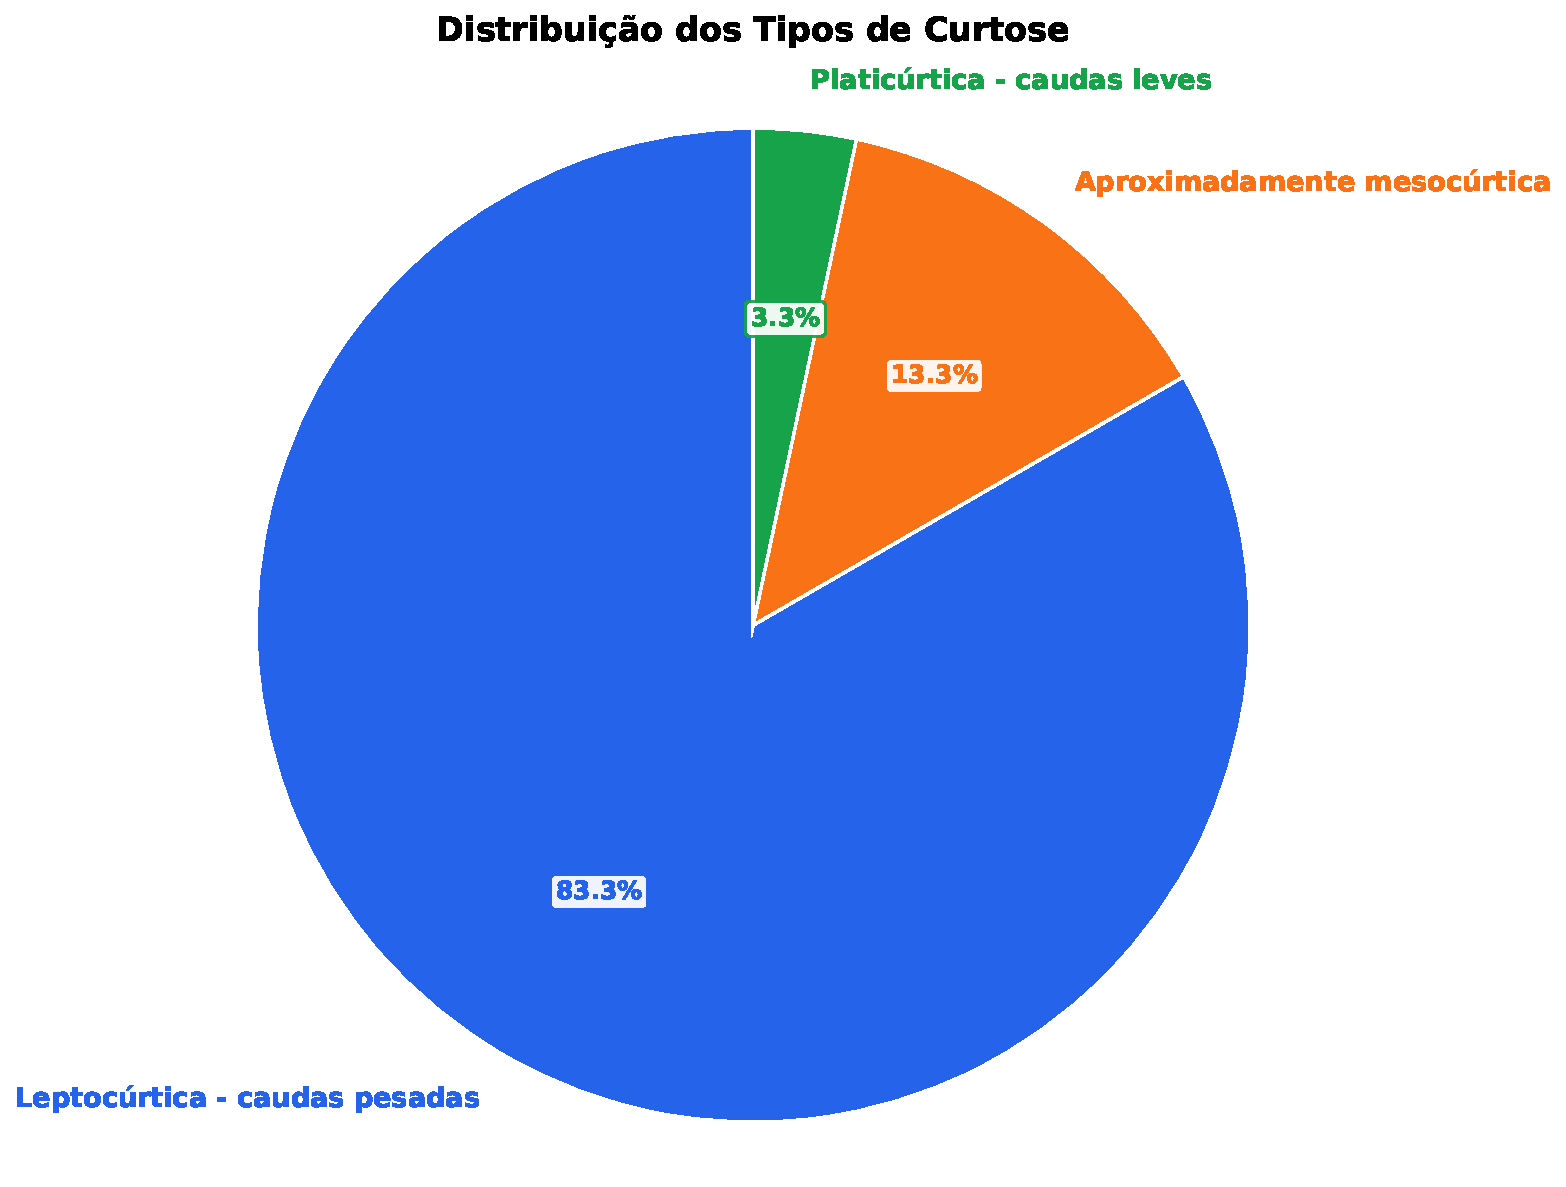
\includegraphics[width=0.75\textwidth]{features_analise_exploratoria/grafico_curtose.pdf}
\caption{Distribuição dos tipos de curtose das features numéricas.}
\label{fig:grafico-curtose}
\end{figure}

% ----------------------------
% Matriz de Pearson
% ----------------------------
\begin{figure}[H]
\centering
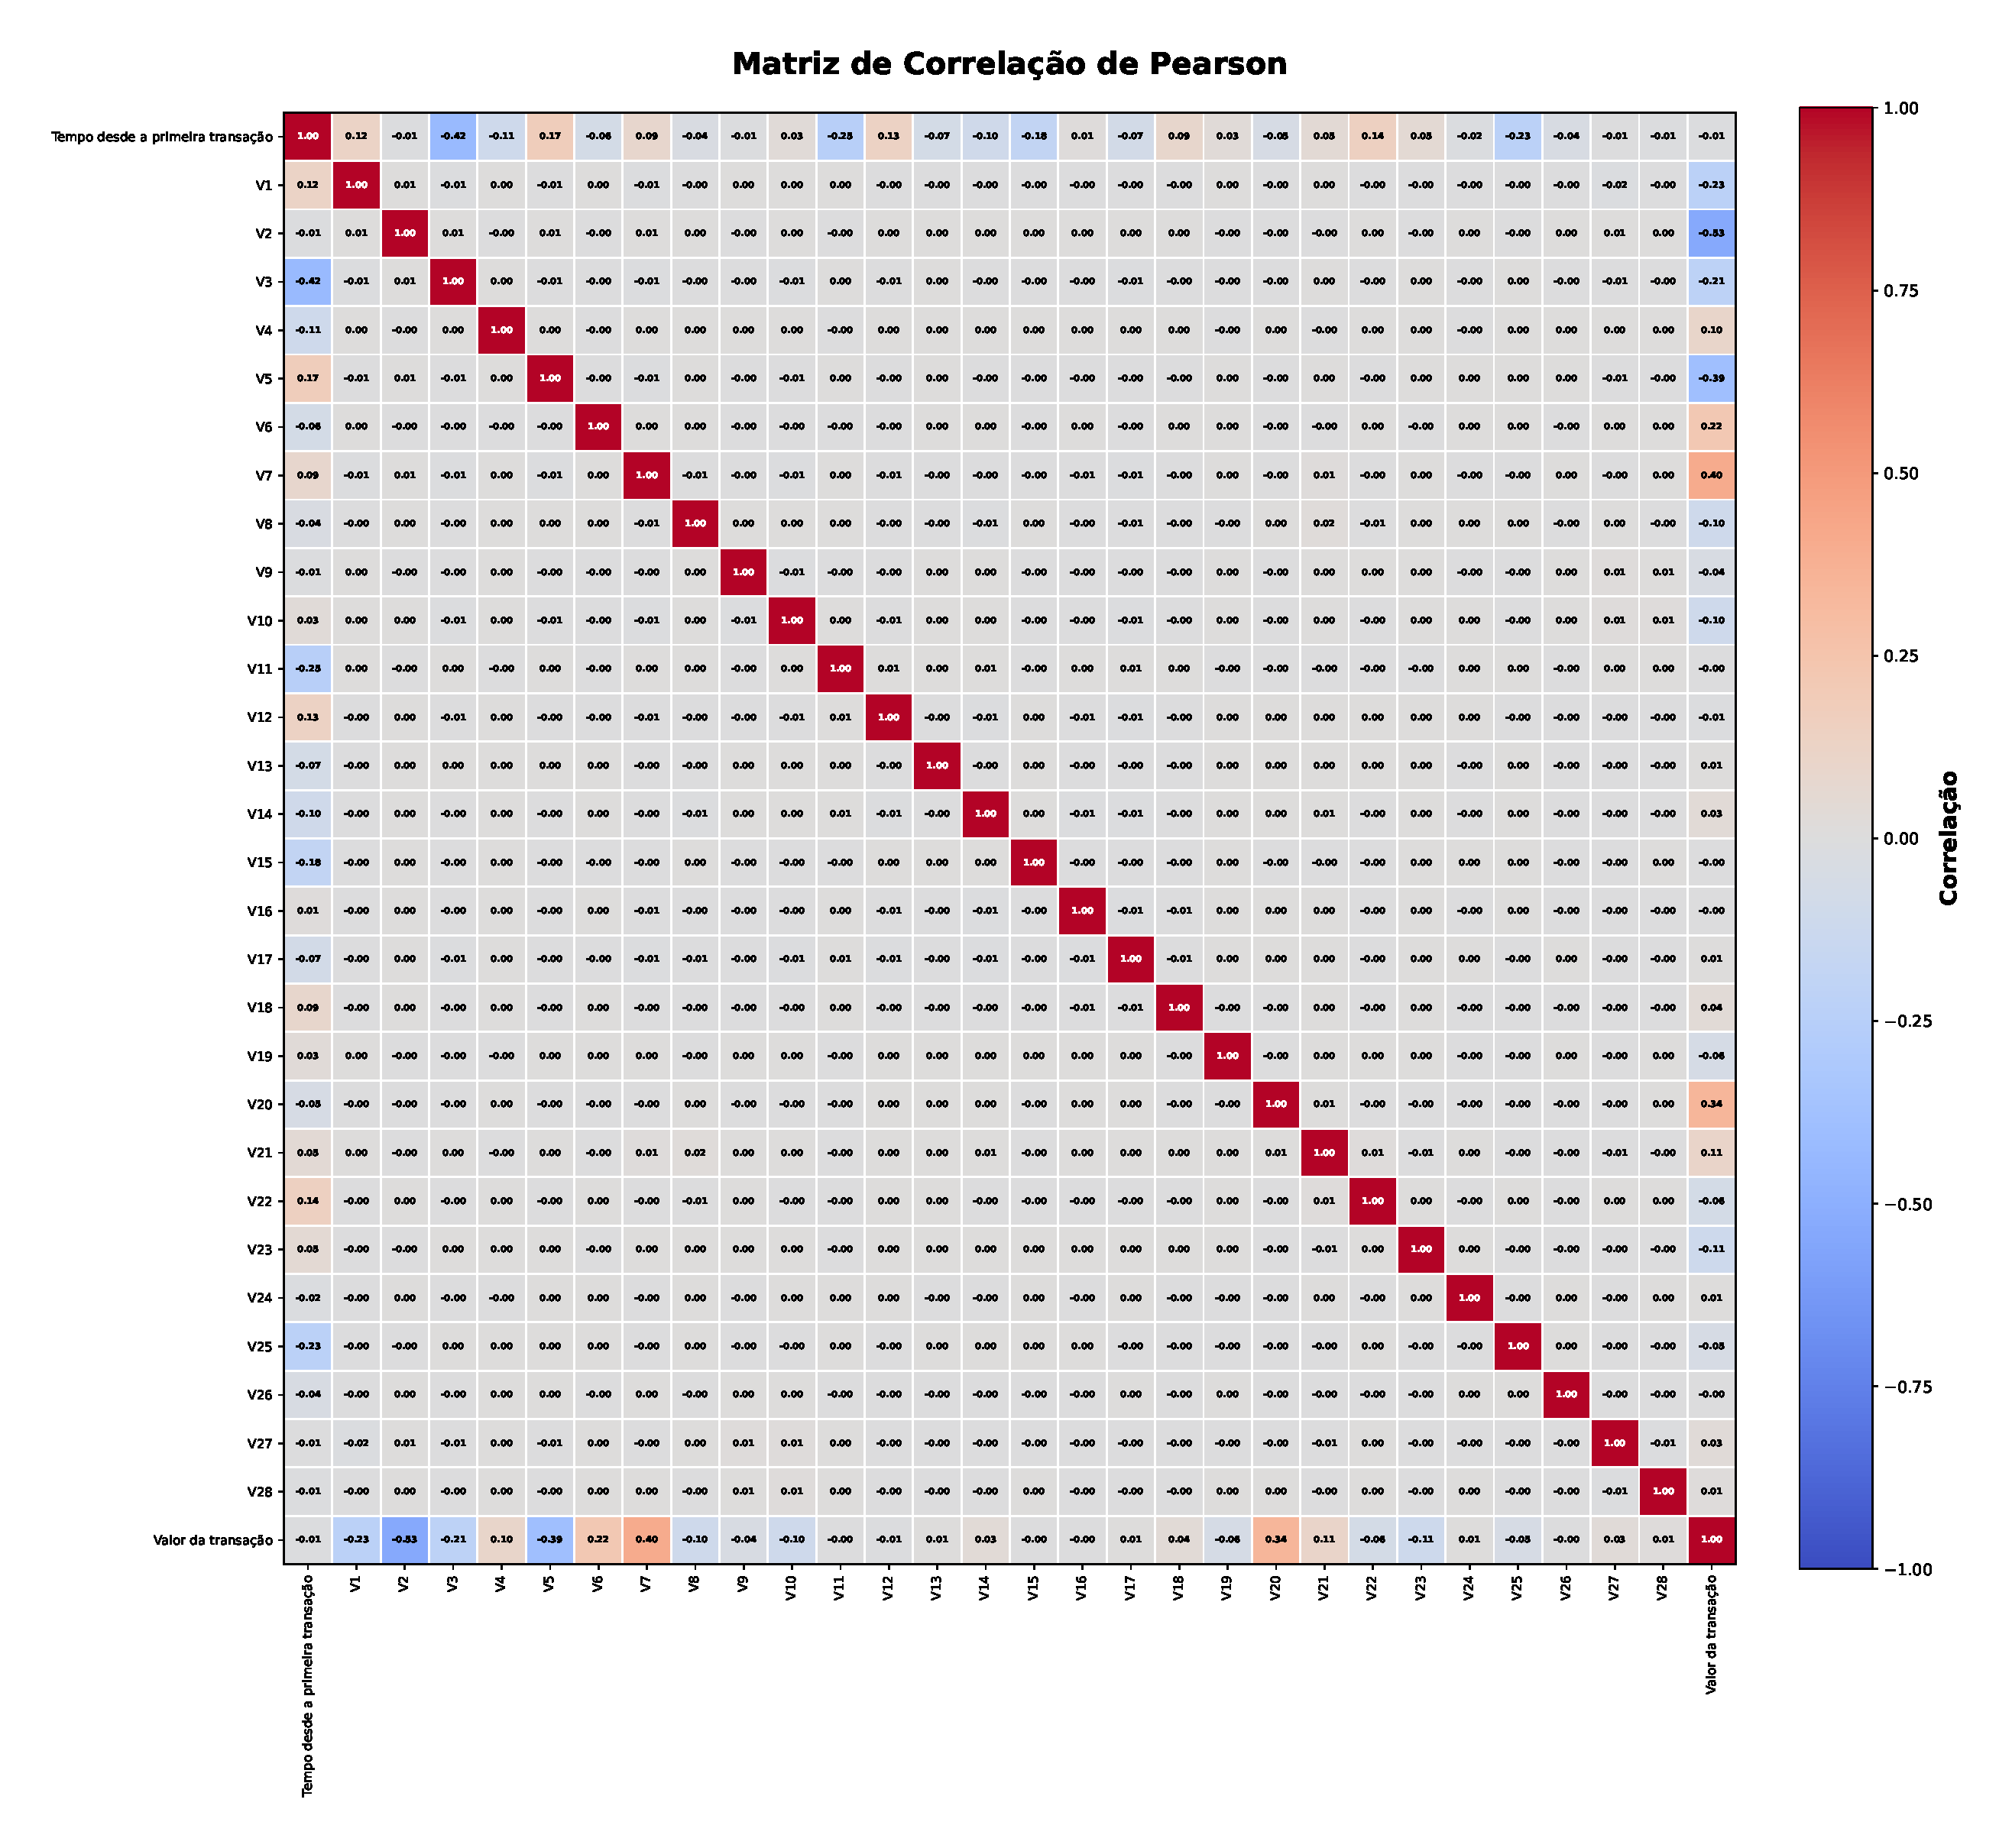
\includegraphics[width=\textwidth]{features_analise_exploratoria/matriz_pearson.pdf}
\caption{Matriz de correlação de Pearson entre as features numéricas.}
\label{fig:matriz-pearson}
\end{figure}

% ----------------------------
% Matriz de Spearman
% ----------------------------
\begin{figure}[H]
\centering
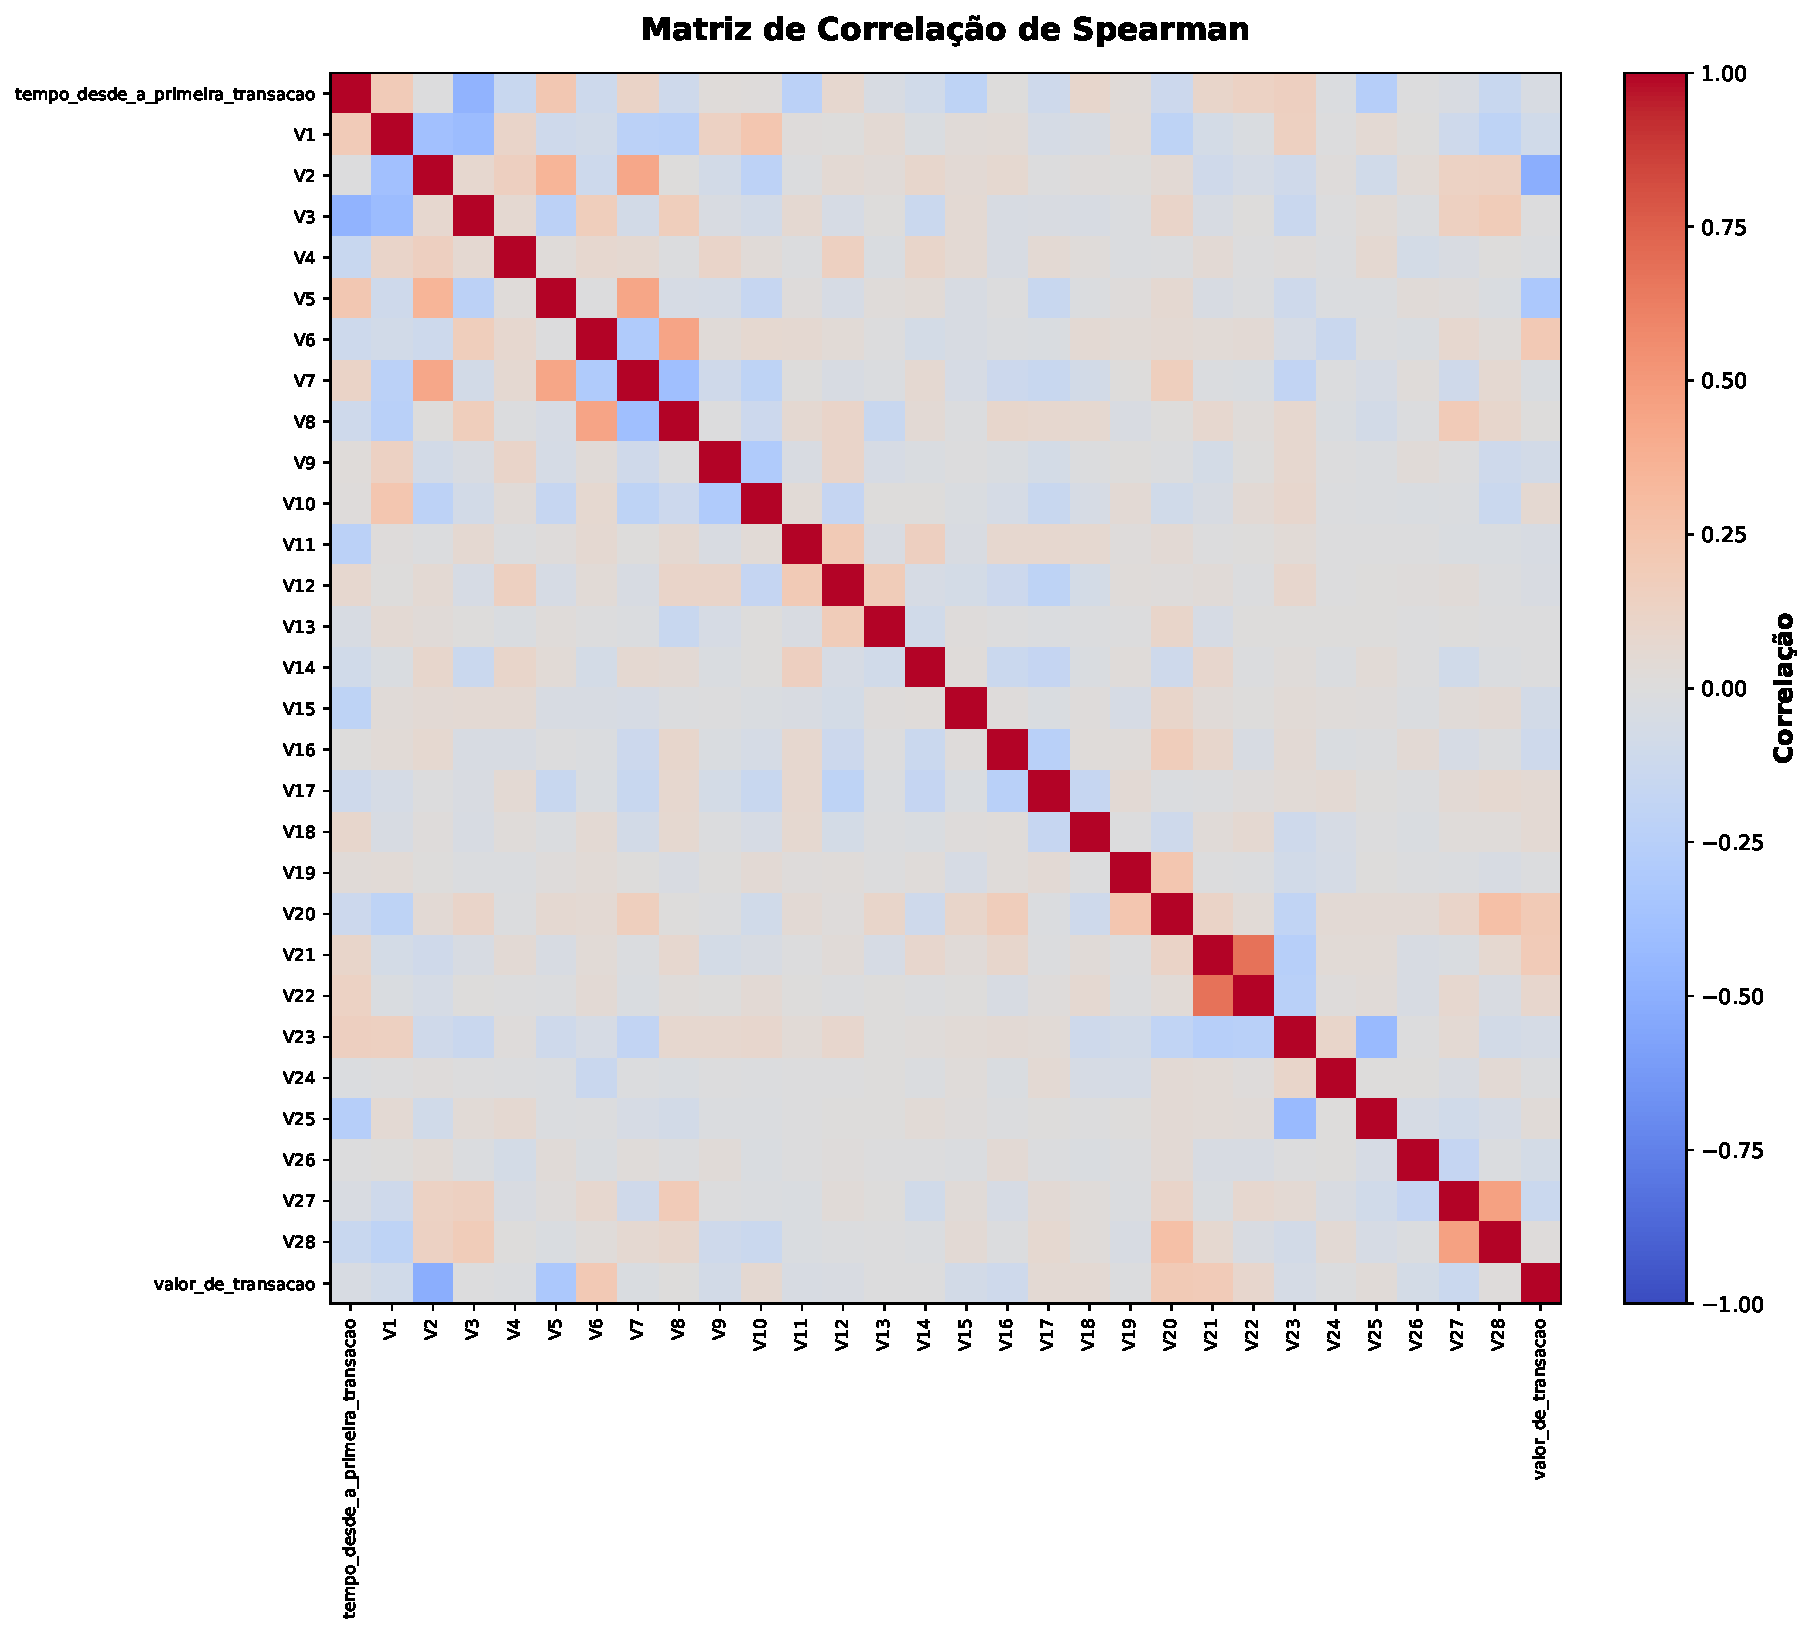
\includegraphics[width=\textwidth]{features_analise_exploratoria/matriz_spearman.pdf}
\caption{Matriz de correlação de Spearman entre as features numéricas.}
\label{fig:matriz-spearman}
\end{figure}
